\documentclass{article}

\usepackage[final]{nips_2017}
\usepackage[utf8]{inputenc} % allow utf-8 input
\usepackage[T1]{fontenc}    % use 8-bit T1 fonts
\usepackage{hyperref}       % hyperlinks
\usepackage{url}            % simple URL typesetting
\usepackage{booktabs}       % professional-quality tables: https://www.ctan.org/pkg/booktabs
\usepackage{amsfonts}       % blackboard math symbols
\usepackage{nicefrac}       % compact symbols for 1/2, etc.
\usepackage{microtype}      % microtypography
\usepackage{graphicx}	% Use pdf, png, jpg, or eps
\usepackage{subcaption}
\usepackage{float}
\usepackage{bm}
\usepackage{amsmath}	
\usepackage{algorithm}
\usepackage[utf8]{inputenc}
\usepackage[noend]{algpseudocode}
%\usepackage{algorithmic}
\title{Document Classification with Reuter50 News Text}

\author{
Muzhe Zeng\\
\texttt{mzeng6@wisc.edu} 
}

\begin{document}
% Use \nicefrac{1}{2}~ to write fraction in line
% Use \label{a_name} under a section to label the number of the section and \ref{a_name} to reference the number in line
% Use ``What you want write'' to write double quotation marks.
% Use In the previous work of Jones et al\[4]. to refer to a paper in the text.
% Use \footnote{What you want to write as a footnote} in the text.
% bold font \textbf{XXX},  italic \emph{XXX}
% Use \begin{itemize}  and \item to make a list


\maketitle

%Furthermore, we also examine each method's performance over a dimension-shrunk feature space. The shrinkage method is PCA + Varimax rotation. A recent paper [1] showed that this technique (\texttt{vsp}) can infer statistical meaningful latent factors, which could be used as good predictors for supervised tasks. Our experiment shows that \texttt{vsp} + supervised learning can speed up the training process significantly with minor loss in accuracy.

\begin{abstract}
This paper utilizes sever supervised machine learning methods to perform document classification task. The involved machine learning methods are logistic regression, support vector machine, and multi-layer perceptions (deep neural network). The goal is to compare these methods and investigate each methods' strengths in terms of accuracy and speed.  The project Github repository is in \url{https://github.com/MuzheZeng/Document-Classification-with-vsp}.
\end{abstract}


\section{Introduction}
Machine learning (ML) is transforming the world's life in all respects. With the growing knowledge in ML area as well as the wide-spread applications, the ML community is expanding at an unprecedented rate. One direct outcome is the production of various ML methodologies. Just like shoppers are usually overwhelmed by the numerous options in the shopping mall and confused about which item is the best to spend money on. ML practitioners are also frequently encountering the question of which ML method to apply or experiment in solving different real-world problems. 

ML methods can be categorized into subgroup in many sense: supervised vs un-supervised learning, parametric vs non-parametric, etc. For supervised learning, the most popular ones include but not limit to linear regression (LR) [1], decision tree, support vector machine (SVM) [2], artificial neural network (ANN) [3]. Each method construct the data model from a different perspectives and come with different model assumptions. The computation strategies and the theory behind them are also distinctly diverse. As the ML community grows, is becomes more and more important to gain knowledge about the comparisons between these ML models.

In this paper, we are comparing three popular supervised learning methods: LR, SVM, and ANN. Text classification is presumably hard and is able to reveal most MLs' weaknesses. Therefore the comparison will be focused on high-dimensional unstructured text dataset and the task document classification. %Also, the ML performance depends not only on the algorithms, but also the features applied in the model. This paper also explore a variant of PCA dimension reduction technique to reduce the high-dimensional nature of text data. To evaluate same set of aforementioned ML methods with different features extracted in the corpora. 

After the introduction section, we will describe the dataset in Section 2. Then we revisit the basics of these three popular ML methods in Section 3. Section 4 summarizes the experiment result and we conclude our paper in Section 5. 

\section{Dataset}

The dataset is collected from UCI: \url{https://archive.ics.uci.edu/ml/datasets/Reuter_50_50}. The dataset is split in halves for training and testing purpose, with 2500 documents each. The response variable is the author of each text, and there are 50 authors (then 50 categorical levels). The response variable is perfectly balanced in both train and test set. 

\newpage

An example of a instance in our training set is displayed below:
\begin{quote}
Drugstore giant Revco D.S. Inc. said Monday it agreed to buy regional chain Big B Inc. in a sweetened takeover valued at \$380 million.
The transaction calls for Twinsburg, Ohio-based Revco to buy all outstanding shares of Big B common stock for \$17.25 per share, up from Revco's unsolicited offer of \$15 per share, which Big B rejected last month.
"We are very excited about the combination of Revco and Big B. I am pleased we were able to bring this process to a fast and successful conclusion," said Dwayne Hoven, president and chief executive officer of Revco.
The deal will ...
\end{quote}

The example above has 677 words and belongs to the writer RobinSidel. The average length of the train set is 488 words and 495 for test set. The names of all the writers (categorical labels) are listed below.
\begin{verbatim}
['AaronPressman' 'AlanCrosby' 'AlexanderSmith' 'BenjaminKangLim'
 'BernardHickey' 'BradDorfman' 'DarrenSchuettler' 'DavidLawder'
 'EdnaFernandes' 'EricAuchard' 'FumikoFujisaki' 'GrahamEarnshaw'
 'HeatherScoffield' 'JanLopatka' 'JaneMacartney' 'JimGilchrist'
 'JoWinterbottom' 'JoeOrtiz' 'JohnMastrini' 'JonathanBirt' 'KarlPenhaul'
 'KeithWeir' 'KevinDrawbaugh' 'KevinMorrison' 'KirstinRidley'
 'KouroshKarimkhany' 'LydiaZajc' "LynneO'Donnell" 'LynnleyBrowning'
 'MarcelMichelson' 'MarkBendeich' 'MartinWolk' 'MatthewBunce'
 'MichaelConnor' 'MureDickie' 'NickLouth' 'PatriciaCommins'
 'PeterHumphrey' 'PierreTran' 'RobinSidel' 'RogerFillion' 'SamuelPerry'
 'SarahDavison' 'ScottHillis' 'SimonCowell' 'TanEeLyn' 'TheresePoletti'
 'TimFarrand' 'ToddNissen' 'WilliamKazer']
\end{verbatim}

The most frequent vocabularies in the train set is:

\begin{figure}[htbp]
  {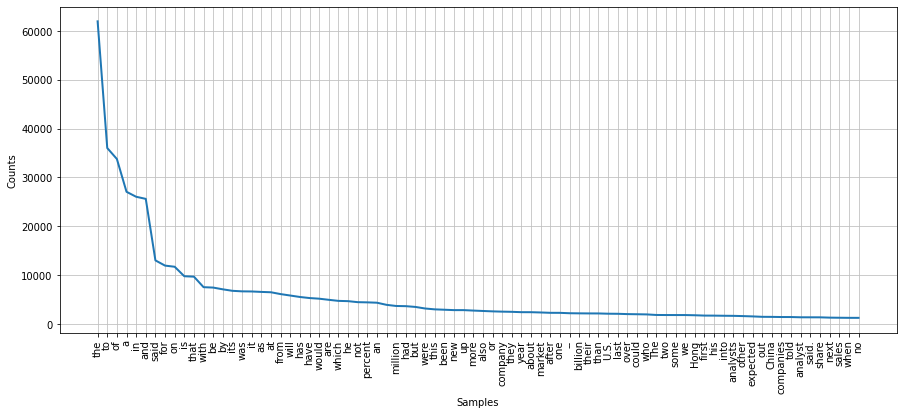
\includegraphics[width=\textwidth]{fd.png}}
    {\caption{Top 80 words appear in the train set. Most of them are stop-words. Our ML experiment will remove these non-informative signals.} \label{fig:year}}
\end{figure}


\section{Methods}

\subsection{Logistic Regression}
For binary logistic regression, the response variable is a two-level categorical column. The generalized linear model language suggests the model relation as

\begin{equation}
z = X \theta = \theta_1 X_1 + \theta_2 X_2 + \cdots + \theta_p X_p. 
\end{equation}

and the probability of response variable $y$ being positive $(=1)$ is 

\begin{equation}
\Pr(y=1) = g(z) = \frac{e^z}{1+ e^z}. 
\end{equation}

The right hand side of Equation (2) is called link function.


\subsection{Support Vector Machine}
SVM is a versatile and powerful supervised ML, which is able to deal with linear or nonlinear classification, regression problems. For regression purpose, SVM aims to fit the largest possible "streets" such that most samples fall within the area between the "streets". The "kernel trick" in the SVM theory facilitates the computation for feature extensions. This is a key step for SVM to handle nonlinearity in the data. Four popular kernel options are: 
\begin{description}
\item[Linear] $K(a,b) = a^Tb)$.
\item[Polynomial] $K(a,b) = (\gamma a^Tb+r)^d$.
\item[RBF] $K(a,b) = \exp(-\gamma\|a-b\|^2)$.
\item[Sigmoid] $K(a,b) = tanh(\gamma a^Tb+r)$.
\end{description}



\subsection{Artificial Neural Network}

Artificial Neural Network (ANN) is the foundation of DL. The model architecture is inspired by the computational neurobiology domain to mimic the signal transportation mechanism among neurons and synapses in the brain. The further development of Back-Propagation (BP) algorithm and automatic differentiation, stochastic gradient descent (SGD), batch normalization, GPR integration, etc, all enable the wide spread application of DL. 

\begin{figure}[htbp]
\centering
  {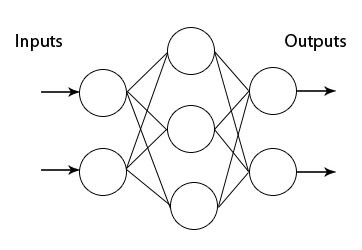
\includegraphics[width=0.4\textwidth]{ann.jpeg}}
    {\caption{A visualization of 3-layer artificial neural network.} \label{fig:ann}}
\end{figure}

%\subsection{Vintage Sparse PCA}
%
%The paper [1] introduces a variant of PCA for dimension reduction purpose. [1] mathematically shows that, \texttt{vsp} can recover the intrinsic low dimension latent factors asymptotically under mild conditions. A key step is the Varimax rotation after the PCA step. 
%
%\textbf{Varimax Criteria.} Given a $n\times k$ matrix $U$, with columns being an orthonormal basis. Varimax finds a $k\times k$ orthogonal matrix $R$ to maximize the sum of the variance of squared loadings of each column:
%\begin{equation} 
%V_U(R) = \sum_{j=1}^{k}\frac{1}{n}\sum_{i=1}^{n}\left([UR]_{ij}^4 - \left(\frac{1}{n}\sum_{\ell=1}^n[UR]_{\ell j}^2\right)^2 \right). 
%\end{equation} 


\section{Experiment}

Logistic regression does not require hyper-parameter tuning step. For SVM, there are: constraint factor ($C$), kernel option. For ANN, there are: hidden layer size, number of layers, activation functions, penalty parameter ($\alpha$), etc. We tune the hyper-parameters by grid search cross validation using only the training set. Eventually, we select the following hyper-parameters:
\begin{description}
\item[SVM] $C=10$, kernel $=$ sigmoid.
\item[ANN] Hidden layer structure $=$ (100, 100), activation function $=$ logistic, $\alpha = 0.1$.  
\end{description}

\newpage

\begin{table}[h]
    \centering
    \begin{tabular}{c|rrr}
    \hline
      Model   & CV accuracy & test accuracy & training time (seconds) \\
    \hline
     Linear Regression & 0.85 & 0.75  & 55\\
     Support Vector Machine & 0.83 & 0.67 & 330 \\
     Artificial Neural Network &  0.87  & 0.76  & 297\\
     \hline
    \end{tabular}
    \caption{Experiment Results. Comparisons of accuracy and speed.}
    \label{tab}
\end{table}


\begin{figure}[htbp]
\centering
  {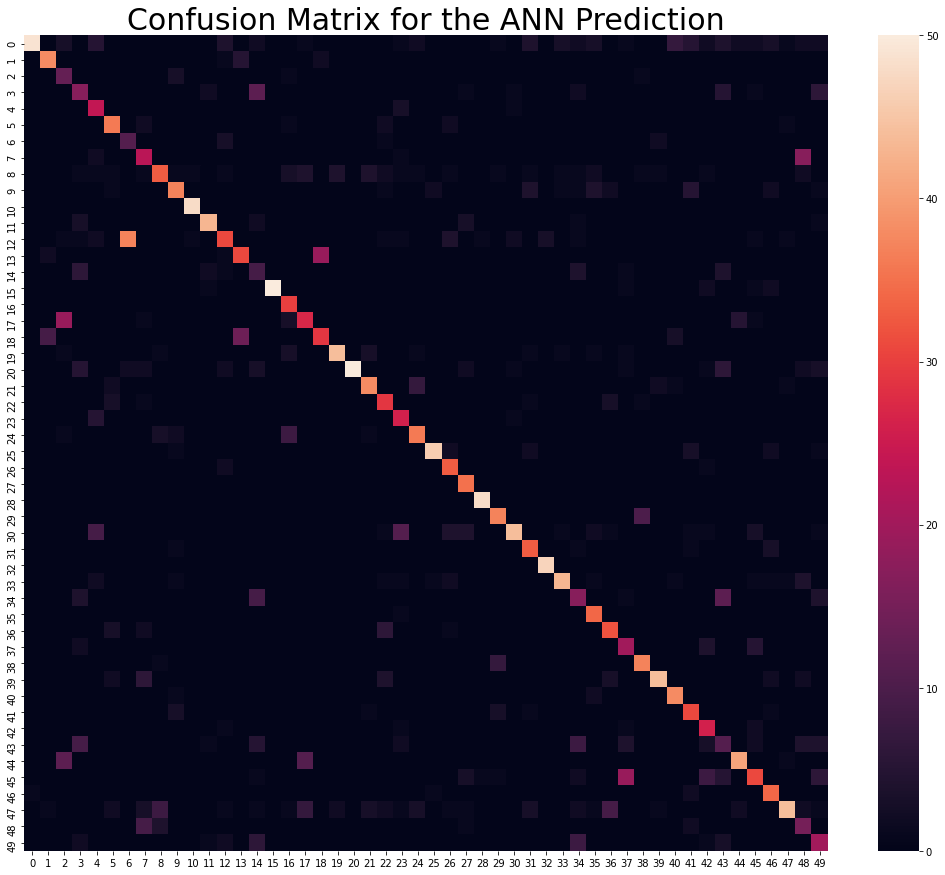
\includegraphics[width=0.8\textwidth]{confusion.png}}
    {\caption{Confusion matrix for the best model over the test set. The lighter-colored tiles have more samples. Off-diagonal tiles are all mis-classified samples.} \label{fig:cf}}
\end{figure}

Table \ref{tab} summarizes the result of the experiment. The winner among these three candidate ML methods is the famous ANN. With accuracy in the test set as high as 76\%, which is much better than random guess (2\%). Machine learning is popular for a reason! LR is slightly worse than ANN in terms of accuracy. SVM performs the worst among the three. In terms of latency, LR is much faster than the other two. If the classification task is designed for a product in which latency is a major concern, then LR will be the best option among the three. If one only cares about accuracy, then ANN is the choice. 

Figure \ref{fig:cf} demonstrates the confusion matrix of the 50 classes. From this matrix we can investigate which authors' writings are easily mis-recognized. Firstly, most weights fall in the diagonal entries, indicating accurate predictions. By looking at the bright off-diagonal tiles, we can see that ANN sometimes mistaken David Lawder as Heather Scoffield, Alexander Smith as Joe Ortiz, Peter Humphrey as Therese Poletti. 

\section{Discussions}
This paper compares three popular machine learning methods in document classification task. The Artificial Neural Network is the most accurate while Logistic Regression is the fastest. With the help of GPU and parallel computing techniques, one can actually get the best of most worlds. However, the difference between cross-validation error rate and the test set prediction error rate implies certain level of over-fitting. In order to improve the models, one might need to expand the grid search in the hyper-parameter spaces. Also, some feature engineering prior work might further strengthen the signal and therefore improve the performance. 

\section*{References}
\medskip
\small

[1] Hosmer Jr, David W., Stanley Lemeshow, and Rodney X. Sturdivant. Applied logistic regression. Vol. 398. John Wiley \& Sons, 2013.

[2] Cortes, Corinna, and Vladimir Vapnik. "Support vector machine." Machine learning 20, no. 3 (1995): 273-297.

[3] Hassoun, Mohamad H. Fundamentals of artificial neural networks. MIT press, 1995.

\end{document}

\section{Dataset}
The dataset is the subset of RCV1. These corpus has already been used in author identification experiments. In the top 50 authors (with respect to total size of articles) were selected. 50 authors of texts labeled with at least one subtopic of the class CCAT(corporate/industrial) were selected.That way, it is attempted to minimize the topic factor in distinguishing among the texts. The training corpus consists of 2,500 texts (50 per author) and the test corpus includes other 2,500 texts (50 per author) non-overlapping with the training texts. For more details, see \href{https://archive.ics.uci.edu/ml/datasets/Reuter_50_50}{this}. 


\section{Algorithms}
I plan to apply these three ML methods to perform document classification task. 
\begin{itemize}
\item Logistic regression [1] with word counts and \texttt{vsp} [2] extracted latent factors.
\item Support vector machine [3] with word counts and \texttt{vsp} extracted latent factors. 
\item Gradient Boosting Decision Trees [4] with word counts and \texttt{vsp} extracted latent factors. 
\end{itemize}
I'll tune the number of latent factors, svm's kernel function + soft threshold, GBDT's tree depth + \#features + iteration steps+ learning rate. I'll use cross-validation to choose hyperparameters and the test set for comparison between models. The evaluation will be the classification accuracy over the test dataset.








\begin{abstract}
Data and computation parallelism are two major high performance computing techniques to bring efficiency. It's beneficial in numerous areas. One of the most popular applications is machine learning. Parallelism could make machine learning models truly scalable. Stochastic Gradient Descent (SGD) and Alternative Direction Method of Multipliers (ADMM) are two popular and powerful learning algorithms that both being intrinsically embedded with distributed computation mechanism. In this paper we are going to implement two styles of parallelism via: 1, Parallel SGD to solve logistic regression problem with OpenACC/OpenMP/MPI. 2, Parallel ADMM to solve LASSO problem with CUDA/Thrust. Our experiments indicate that hybrid parallelization could gain more than 2000x speed up compared with sequential programming. \\
Team github repository: https://git.cae.wisc.edu/git/me759-muzhe
\end{abstract}

\section{General Information}
\begin{itemize}
\item Department of Statistics.
\item PhD 2nd year.
\item \begin{enumerate}
	\item Muzhe Zeng (Team Leader)
	\item Yanzheng Li
	\item Yudong Chen
	\end{enumerate}
\item Prof. Karl Rohe
\end{itemize}



\section{Project Statement}
There are three major flavors of parallelism: data parallelism, computation parallelism and model parallelism. Data parallelism is to distribute the training data to different computing nodes and update parameters on each local computing node. Then send the updated parameters to a global parameter server and merge the result. Finally, broadcast the globally updated parameters. Computation parallelism is to perform computation (vector, matrix calculations) in parallel fashion, mostly leveraging GPU computing techniques to accelerate the process. Model parallelism is to distribute the different parts of  the machine learning model to each computing node. Each produce enhancement in code performance in different fashions. Model parallelism is rarely used it will not be the interests of our paper. This paper will focus on two parts: 
\begin{enumerate}
\item Data parallelism on logistic regression problem with openMP/openACC/MPI.
\item Computation parallelism on Lasso problem with CUDA/Thrust/Cublas.
\end{enumerate}

Logistic regression is a classical binary prediction linear model. With solid statistical theory background, it is able to give satisfactory estimation in many classification problems. Logistic regression is basically solving this problem: 
\begin{equation} \label{eq:logistic}
y_i \sim Bernoulli(p_i), \quad p_i = \sigma(\theta^{T}x_i), \mbox{ where } \sigma(a) = 1/(1+\exp(a)). 
\end{equation}

The goal is to recover $\theta$ based on observations of $y$ and $x$. With good estimation of $\theta$ we are able to predict $y$ when new data $x$ comes in. There are many efficient iterative algorithm to solve this model. We are going to implement with Stochastic Gradient Descent (SGD). And further deploy data parallelism with Message Passage Interface (MPI). And the meantime accelerate the process with openMP and openACC.

Lasso problem is one of most popular machine learning topics and is still being studied intensively. It was originally formulated for simplification of ordinary least square regression problems by introducing L1-norm penalty. Lasso performs both regularization and variable selection to capture true underlying signal and improve the prediction accuracy and interpretability of the model. We illustrate Lasso explicitly as the following optimization,
\begin{equation} \label{eq:lasso}
\underset{x\in \mathbb{R}^m}{minimize}\quad f(x) := \frac{1}{2}||Ax-b||_{2}^{2} + \lambda||x||_{1},
\end{equation} 

with $A\in \mathbb{R}^{n\times m}, b\in \mathbb{R}^n$. In recent decades Lasso problem has been investigated quite throughly in numerous literatures. It turns out that Lasso produced empirically and theoretically, statistically and numerically valuable perspectives in machine learning community.

Lasso optimization problem involves L1-norm, which is convex but non-smooth function. Typical gradient methods are not available in this scenario. One natural approach is subgradient methods. However, subgradient is at best converging at rate of $\log n / \sqrt{n}$ in theory and performs bad in empirical studies. A better alternative method is proximal gradient descent (PGD) which is powerful in regularized optimization problems. Another famous algorithm that could deal with various regularized optimization problems is alternating direction method of multipliers (ADMM). This algorithm takes the form of a decomposition-coordination procedure, in which the solutions to small local subproblems are coordinated to find a solution to a large global problem. ADMM could be viewed as an attempt to blend the benefits of dual decomposition and augmented Lagrangian methods for constrained optimization. 

We will implement both sequential and parallel version of PGD to address Lasso problem in later sections. ADMM for Lasso requires taking inverse of a large matrix. Considering the complexity of normal matrix inversion operation is $O(n^3)$, which is too costly when $n$ is huge. We only bring ADMM in Cuda/Thrust into list of methods for comparison.

The reason drives me to chose this project is the trend of parallel machine learning methodologies. In terms of large scale data science, there are multiple ways of breaking computation bottlenecks. Parallel computing is one of the hottest trend. SGD and ADMM are intrinsically suitable for parallelism. I've been reading literatures since two years ago and didn't have chance and resources to implement it, until now. 

\section{Solution Description}
\subsection{Logistic Regression}
\subsubsection{SGD with OpenACC}
Using OpenACC in SGD algorithm
Besides adding general syntax in the code we want to parallel in SGD algorithm . Several other aspects are worth pay attention to. 
\begin{enumerate}
\item In the compile script, we do not include the "-ta=tesla:managed" option. The data size and operation is far more complex in SGD than the Gaussian Blur image filter. So coping too much data to managed memory would cause the “out of memory” error.
\item If we not include "-ta=tesla:managed" option in SGD algorithm. Sometimes the compiler don’t know about the size of matrix copy/copyin/copyout to GPU. So we need to explicitly add "copyin(list[:])" clause.
\item In SGD algorithm. I include all the epoch iteration in the parallel region. The compiler will automatically pick which loop are paralleled and which are not without specifing "collapse" and "seq"
\end{enumerate}

\subsubsection{SGD with OpenMP}
In the SGD algorithm, we parallel the for loop of sum over the product of data matrix and weight matrix using OpenMP reduction, and parallel the update of weight based on the cross entropy loss.

\subsubsection{SGD with MPI}
Running a Slurm job on Euler can has at most 4 nodes and 8 cores per node, which can make use of 4 nodes running SGD algorithm on different data batch and on each node calculation can use OpenMP to parallelize. Every 16 epoch, weight matrix from all the other rank are collected by rank 0 using mpi reduce. After averaging weight matrix, the matrix are broadcasted to the other rank by using mpi broadcast. Averaging the weight matrix every 16 epoch can reduce the overhead of communication between rank every epoch with slightly inference on convergence rate. But we did not finish this implementation due to time limit. The following is the pesudocode.

\begin{algorithm}[H]
\caption{Stochastic Gradient Descent on MPI(Expected)}\label{SGD_MPI}
\begin{algorithmic}[1]
\State{\textbf{Initialize} X,w,y}
% \For{$k = 1,2,\cdots,m$}
\State{Start MPI}
\State{Create and initialize the localWeight matrix:(localWeight)}
\For{$i=1,2,\cdots,epoch/16$}
    \For{$16\ times$}
        \State{SGD algorithm updating localWeight using  data only in that batch}
    \EndFor
    \If{$rank = 0$}
        \State{reduce localWeight from all rank}
        \State{averaging localWeight }
        \State{broadcast to all the other rank.}
    \EndIf
\EndFor
\end{algorithmic}
\end{algorithm}

\subsection{LASSO}
We generated $A$'s elements randomly from $[-10, 10]$ and $x_{true}$ being a m-vector that has 1's in first $[\frac{m}{200}]$ entries and 0's elsewhere. $b = Ax_{true}$ and the initial value for $x$ is random numbers between $[-0.1, 0.1]$.


\subsubsection{Proximal Gradient Descent}
To introduce PGD we need to talk about Moreau envelop first. It is defined as
\begin{equation} \label{eq:moreau}
M_{\lambda, h}(x) := \underset{u}{\inf}\{h(r)+\frac{1}{2\lambda}||u-x||^{2}_2\} = \frac{1}{\lambda}\underset{u}{\inf}\{\lambda h(u) + \frac{1}{2}||u-x||^{2}_2\}.
\end{equation}
The proximal-operator of the function $\lambda h$ is value of $u$ that achieves the infimum of (2).
\begin{equation} \label{eq:proximal}
\mbox{prox}_{\lambda h}(x) := \mbox{$\arg$}\underset{u}{\min}\{\lambda h(u) + \frac{1}{2}||u-x||^{2}_2\}.
\end{equation}

For the line-search choice, we employ Armijo backtracking strategy along the projection arc, in which we choose an $\alpha > 0$ and take the step $\alpha_k$ to be the first element in the sequence $\alpha, \beta\alpha, \beta^2\alpha,...$ for which the following condition is satisfied,
\begin{equation}
f(x_k(\beta^m\alpha)) \leq f(x_k) + c_1 \nabla f(x_k)^{T}(x_k(\beta^m\alpha)-x_k),
\end{equation}
with the $x$ update as 
\begin{equation}
x_{k+1}  = \mbox{prox}_{\alpha_k\lambda \phi}(x_k - \alpha_k\nabla f(x_k)),
\end{equation}
where $\phi$ is L1-norm function.

\vspace{2mm}
To put together, we obtain the following PGD algorithm for solving Lasso problem (2). 
\begin{algorithm}[H]
\caption{Proximal Gradient Descent (PGD)}\label{PGD}
\begin{algorithmic}[1]
\State{\textbf{Initialize} $\mathbf{x}^{(0)} \mbox{ randomly}, k = 0, \alpha_0 = 1, c_1 = 0.5, \beta = 0.8$}
%\For{$k = 1,2,\cdots,m$}
%\State{}
\Repeat 
\State{Linesearch $\alpha_{m,k}$ until Armijo criteria is satisfied at $x^{(k)}$.}
\State{$x^{(k+1)} = S_{\lambda \alpha_{m,k}}(x^{(k)} + \alpha_{m,k}A^{T}(b - Ax^{(k)}))$}
\Comment{Gradient descent part}
\State{$k = k + 1$}\Comment{Update number of iterations}
\Until{$ ||x^{(k+1)} -x^{(k)}||_2 / ||x^{(k+1)}||_2 < \varepsilon$ or $k > K$}\\
\Return{$x^{(k)}$}
\end{algorithmic}
\end{algorithm}

To be more specific, the $S_{a}(x)$ is soft thresholding function with parameter $a$,
\begin{displaymath}
[S_a(x)]_i = \left \{ \begin{array} {ll}
x_i - a & \textrm{if $x_i > a$,}\\
0 & \textrm{if $-a \leq x_i \leq a$,}\\
x_i + a & \textrm{if $x_i < -a$,}\\
\end{array} \right.
\end{displaymath}

\textbf{Implementation} We store matrices and vectors in float arrays (device float vector) while implementing sequentially (in parallel). We initialize every thing with same values so the estimations of $x$ should be almost the same for both versions (slight difference is expected when the dimension is high because of the rounding errors). We list the implementation details of the important functions used in this part of algorithm below.

\begin{description}
\item[inner-product] Sequential: \textsf{innerProd()}, with one for loop. Parallel: one liner of \textsf{thrust::transform()}.
\item[vector norm] Sequential: \textsf{vec\_norm()}, with one for loop. Parallel: \textsf{two\_norm()}, use \textsf{thrust::transform()} with functor \textsf{square} to sum up squared values of each element in a device vector.
\item[matrix multiplies vector] Sequential: \textsf{matMultiply()}, with two nested for loops. Parallel: Calculate element-wise multiplications with kernel function \textsf{matrixMultiplication()} and cached the matrix (same size as original matrix), calculate the row-wise sum of this matrix with \textsf{matVec} using \textsf{thrust::reduce\_by\_key()}. 
\item[matrix transpose] Sequential: \textsf{transpose()}, with two nested for loops. Parallel: \textsf{transpose()} with kernel function \textsf{transp()}.
\item[soft threshold operator] Sequential: \textsf{softVec()}, with one for loop. Parallel: \textsf{thrust::transform()} with functor \textsf{soften}.
\item[$f(x)$] Sequential: \textsf{f()} with combined use of \textsf{matMultiply()} and for loop. Parallel: \textsf{lasso()} with combined use of \textsf{matVec()}, \textsf{thrust::transform()} and \textsf{one\_norm()}.
\item[$\nabla f(x)$] Sequential: \textsf{fdiff()}. Parallel: \textsf{dlasso()}.
\item[$x$ update] Sequential: \textsf{xx()} with combined use of \textsf{matMultiply()}, \textsf{transpose()}, \textsf{softVec} and a for loop saxpy operation. Parallel: \textsf{xx()} with combined use of \textsf{matVec()}, \textsf{transpose()} and three \textsf{thrust::transform()} for minus, saxpy, soft thresholding operations.
\end{description}
  
\textbf{Remarks} The most computationally heavy part is matrix-multiply-vector operation, which is inside more than one functions and has been repeatedly used in every iteration of the learning process so this is the first place I optimized into parallel fashion. For the kernel execution configuration, I set 512 threads in one block and 2-dimension block grid with size of $n \times m/512$. The same configuration is used for transpose operations.  


\subsubsection{Alternative Direction Method of Multipliers}

For generic constrained convex optimization problem
\begin{equation}
\mbox{minimize} \quad g(x) + h(x) 
\end{equation}

ADMM rewrites the problem as
\begin{eqnarray*}
&& \mbox{minimize} \quad g(x) + h(z) \\
&& \mbox{subject to} \quad x = z.
\end{eqnarray*}

With scaled dual variable, the Augmented Lagrangian is
\begin{equation}
\mathcal{L}_{\rho}(x,z,u) = g(x) + h(z)+\frac{\rho}{2}||x-z+u||^{2}_{2}. 
\end{equation}

The ADMM update for it is
\begin{eqnarray*}
x^{(k+1)} &=& \underset{x}{\arg\min}(g(x) + \frac{\rho}{2}||x-z^{(k)}+u^{(k)}||^{2}_{2}, \\
z^{(k+1)} &=& \underset{z}{\arg\min}(h(z) + \frac{\rho}{2}||x^{(k+1)}-z+u^{(k)}||^{2}_{2},  \\ 
u^{(k+1)} &=& u^{(k)} + k^{(k+1)} - z^{(k+1)}.
\end{eqnarray*}

To put it into Lasso problem's setting (let $g(x) = ||Ax-b||_{2}^{2}/2, h(z) = \lambda||x||_1$), we obtain the following algorithm,

\begin{algorithm}[H]
\caption{Alternative Direction Method of Multipliers (ADMM)}\label{ADMM}
\begin{algorithmic}[1]
\State{\textbf{Initialize} $x^{(0)}, z^{(0)} \mbox{ randomly}, k = 0, \rho = 1$}
%\For{$k = 1,2,\cdots,m$}
%\State{}
\Repeat 
\State{$x^{(k+1)} = (A^{T}A+\rho I)^{-1}(A^{T}b+\rho(z^{(k)}-u^{(k)}))$} 
\Comment{Update $x$}
\State{$z^{(k+1)} = S_{\lambda/\rho}(x^{(k+1)}+u^{(k)})$} 
\Comment{Update $z$}
\State{$u^{(k+1)} = u^{(k)} + x^{(k+1)} - z^{(k+1)}$}
\Comment{Update $u$}
\State{$k = k + 1$} \Comment{Update number of iterations}
\Until{$||x^{(k+1)} -x^{(k)}||_2 < \varepsilon$ and $ ||z^{(k+1)} -z^{(k)}||_2 < \varepsilon$ or $k > K$}\\
\Return{$x^{(k)}$}
\end{algorithmic}
\end{algorithm}

\textbf{Implementation} We store matrices and vectors in device float vector while implementing in parallel. Since the matrix inversion is too intractable in sequential computing, we only compare results of PGD with ADMM in parallel. We initialize every thing with same values as PGD settings. We list the implementation details of the important functions used in this part of algorithm below.

\begin{description}
\item[inner-product] Same as PGD in parallel.
\item[two norm] Same as PGD in parallel.
\item[matrix transposition] Same as PGD in parallel.
\item[matrix multiplication] \textsf{gpu\_blas\_mmul()} using \textsf{cublas\_v2} library (key function: \textsf{cublasSgemm()}).
\item[matrix inversion] \textsf{invert()} using \textsf{cublas\_v2} library (key function: \textsf{cublasSgetrfBatched()}, \textsf{cublasSgetriBatched()}).
\end{description}

\textbf{Remarks} Notice the matrix inversion result could be cached for future usage, we only have to do it once at the beginning. Same as matrix-matrix multiplications. The remaining computation is focused on matrix-vector multiplication, since we do not need to do line search step here, so we are expecting much smaller computation burden compared with PGD algorithm. We used \textsf{nvprof} for profiling throughout the experiment.

One thing to keep in mind is that \textsf{cublas\_v2} by default is column major instead of our row major fashion. That is to say, to perform matrix multiplication $XY$, we need to put $X^{T}, Y^{T}$ into arguments instead of original matrix $X, Y$. 

\section{Results Overview}

\subsection{Data Parallelism in SGD}

\begin{figure}[H]
\centering
\includegraphics[width=0.55\textwidth]{sgd.png}
\caption{Scaling Analysis in terms of data size of sequential programming, openACC and openMP. OpenMP is the best among these three.}
\label{logistic}
\end{figure}

The speed of openMP implementation of SGD is similar to that of parallel implementation of SGD when data size is below $2^{13}$, afterwards, the difference of time taken between these two implementation doubles when data size increase by order of 2. The gap between the time taken by openACC implementation of SGD and time taken by parallel implementation of SGD is growing at order of 2 when the data size increased by order of two. That may due to that the overheads created by data movement is outweighed the acceleration from parallelism and when data size increases, the overheads becomes more and more dominant.



\subsection{Computation Parallelism in PGD, ADMM}

One of the reason that Lasso is attracted to many scholars is that it could deal with high dimensional case with $n < m$. But large $m$ will result in much longer time consumption. Therefore we fix $m=512$, and perform scaling analysis on increasing $n$. We selected $n = 2^k$ with $k = 9, 10, 11, ..., 15$ for PGD experiments and $k = 9,10, ... 20$. The result is shown below. 

\begin{figure}[H]
\centering
\includegraphics[width=0.55\textwidth]{scale.png}
\caption{Scaling Analysis in terms of $n$ of sequential Proximal Gradient Descent (green), parallel Proximal Gradient Descent (red) and parallel Alternative Direction Method of Multipliers (blue). Parallel ADMM beats the other two approaches drastically.}
\label{lasso}
\end{figure}

Each implementation of same $n, m$ combination the lasso problem is the same (identical $A, b, \lambda$ values). Since some initial values of $A, b, \lambda$ requires more iterations than others, so we are not seeing strictly monotonous increasing trend of some curves (i.e. sequential curve). But the difference among three methods is clear. 

We can see that parallel PGD is about 2 order faster than sequential PGD at the beginning, and is 4 order faster when $n$ rises to $2^{15}$. Parallel ADMM is almost 2 order faster than parallel PGD when $n=2^9$ and is scaling very well. The blue curve is almost not changing before $n$ rises to $2^{15}$ (more than 4 order faster than parallel PGD and 8 order faster than sequential PGD). For $n$ larger than $2^{15}$, parallel ADMM could easily solve Lasso problem in short amount of time. As a matter of fact, it took less time for parallel ADMM to finish $n=2^{20}$ than parallel PGD to finished $n=2^{9}$. Compare with sequential PGD, parallel ADMM overall gained 2463x speed up in combination of $n=2^{15}, m=512$. So we witnessed a huge speedup of ADMM in CUDA incorporating parallel computation and algorithmic advantage. 


\section{Deliverables}
\subsection{Data Parallelism in SGD}
To examming SGD’s algorithm on sequential code, OpenMP, OpenACC. Go to “/testing/logistic” folder. “SGD\_SEQ.c” is the source code for sequential and OpenACC code. “SGD\_OpenMP.c” is the source code for OpenMP code. “build.sh” is used to generate executable. “run.sh” is the script to run these code and the output is going to “run.out”;

Compile codes for OpenMP, OpenACC, sequential implementations are
\begin{verbatim}
module load pgi/18.10
\$CC -O3 -fopenmp -std=c11 -lm -lgomp SGD_OpenMP.c ../../../randoms/randoms.c -o SGD_OpenMP
\$CC -fast -O3 -c11 -lm SGD_SEQ_OpenACC.c ../../../randoms/randoms.c  -o SGD_SEQ
\$CC -fast -O3 -ta=tesla:ccall -Minfo=accel -c11 -lm SGD_SEQ_OpenACC.c  ../../../randoms/randoms.c  -o SGD_OpenACC
module unload pgi/18.10
\end{verbatim}

To run the executables, argument configurations are:
\begin{verbatim}
./SGD_SEQ $instance Number $weight dimension  $epoch 
./SGD_OpenACC $instance Number $weight dimension  $epoch
./SGD_OpenMP $instance Number $weight dimension  $epoch $number of threads on OpenMP
\end{verbatim}

With output information: 1.norm difference, 2. time consumption (ms), for each executable. 

\subsection{Computation Parallelism in PGD, ADMM}
To reproduce this part of results, you should got to directory “\textbf{test/lasso}” and run the script "\textbf{run\_lasso.sh}". Firstly compile with the following statements (already uploaded in bash file "\textbf{test/lasso/build\_lasso.sh}") and generate three executable files: test1, test2, test3.
\begin{verbatim}
module load cuda/10.0
nvcc -ccbin $CU_CCBIN --std c++14 -lm sequential_prox.cu -o test1
nvcc -ccbin $CU_CCBIN --std c++14 -lm parallel_prox.cu -o test2
nvcc -lcublas -ccbin $CU_CCBIN --std c++14 -lm parallel_admm.cu -o test3
module unload cuda/10.0
\end{verbatim}

For PGD codes, you should run the executables \textsf{test1}, \textsf{test2} with arguments: $n, m, \lambda$. For ADMM code you should run executable \textsf{test3} with arguments: $n, m, \lambda, \rho$. For example, after compilation you could sbatch the following lines.
\begin{verbatim}
./test1 1024 512 0.5
./test2 1024 512 0.5
./test3 1024 512 0.5 2
\end{verbatim}

You shall expect the following results (might expect small difference in the relative error values and the time cost). Here relative error is the relative difference between estimation and true $x$. The time refers to inclusive timing.
\begin{verbatim}
sequential PGD:
relative error: 2.62001e-05, time elapsed: 50554 ms.
parallel PGD:
relative error: 0.00096995, time elapsed: 9212.43 ms.
parallel ADMM:
relative error: 1.37713e-06, time elapsed: 328.832 ms.
\end{verbatim}

\textbf{Remarks} You should run with argument $n, m$ both be multiples of 512. You don't want $m$ to be too large since it's computationally heavy. $m$ being 512 or 1024 is good choice. Typical choice for $\lambda$ is in between 0.1 and 0.9. $\rho$ should not be too small. For our testing $\rho=2$ is behaving well. If the accuracy go south, you should increase $\rho$ by a factor of 10. 

\section{Conclusions and Future Work}

In scaling analysis of SGD, given the parameter used, the performance of openMP implementation is best, then is the sequential implementation and the worst is openACC. The reason openACC is slower than sequential implementation is that openACC requires movement of data between host and device. We used a long weights array and a long instance array. The overheads createed by data movement has outweighed the acceleration by parallelism. If the epochs is sufficiently large, the throughput of openACC would be better than sequential implementation. Then openMP implementation has shown a much better performance. The MPI implementation is incomplete because of time limitation. MPI is actually a very good fit for parallelizing logistic regression with SGD algorithm. The data instances could be distributed among nodes and update weights locally. We expected a quicker convergence when MPI version is correctly implemented. The difficulties in MPI implementation is the asychronized-style updates of the parameters on the global server. We hope in our future work, we could have correctly implement it. In addition, in the future work, we also hope to realize the model parallelism of Neural Network, based on our experiences in building a paralleled version of logistic regression.

As for Lasso problem, Proximal Gradient method is a special projection gradient method that enjoys many good theoretical properties. It does not require matrix inversion computation in Lasso problem. However the line-search procedure makes it less advantageous than Alternative Direction Method of Multipliers. Our experiment validated that.

ADMM's power is not fully explored yet. There is a lot more to leverage its intrinsic parallel mechanism. For Lasso problem (2). If $n$ is too large to be tractable, we could split the model across examples, 

\begin{equation}
A = \begin{pmatrix} A_1 \\ A_2 \\ \vdots \\ A_N \end{pmatrix}, b = \begin{pmatrix} b_1 \\ b_2 \\ \vdots \\ b_N \end{pmatrix} 
\end{equation}

Then we could put the model into consensus form:
\begin{eqnarray}
&& \mbox{minimize} \quad \sum_{i=1}^{N} \frac{1}{2}||A_i x_i - b_i||^{2}_2 + \lambda||z||_1, \\
&& \mbox{subject to} \quad x_i - z = 0, \quad i=1,...,N.
\end{eqnarray}

This yields distributed algorithm,
\begin{eqnarray}
x^{(k+1)}_i &=& \underset{x_i}{\arg\min}(\frac{1}{2}||A_i x_i - b_i||^{2}_2  +\frac{\rho}{2}||x_i-z^{(k)} +u_i^{(k)}||^{2}_{2}) \\
z^{(k+1)} &=& S_{\lambda/\rho N}(\bar{x}^{(k+1)} + \bar{u}^{(k)}) \\
u_{i}^{(k+1)} &=& u_{i}^{(k)} + x_{i}^{(k+1)} - z_i^{(k+1)}
\end{eqnarray}

Update for $x$ has analytical solution:
$$ x^{(k+1)} := (A_i^T A_i + \rho I)^{-1}(A_i^T b_i + \rho(z^k - u_i^k)). $$

If $m$ is extremely large, the matrix inversion operation will be expensive. There will be similar distributed ADMM algorithm to split $A$ across features. These are all interesting and promising tasks to explore in the future. In this case each $x_i$-update is a lasso problem with much smaller number of variables, which can be solved using any single processor Lasso method.



\section*{References}
\medskip
\small

[1] Stephen, B. \ \& Neal P., \ \& Eric, C. \ \& Borja, P. \ \& Janathan, E. \ (1998) Distributed Optimization and Statistical Learning via the Alternative Direction Method of Multipliers. {\it Foundations and Trends® in Machine learning} {\bf 3}(1):1-122.

[2] Parikh, Neal, \ \& Stephen Boyd. (2014) Proximal algorithms. {\it Foundations and Trends® in Optimization} 1.3 (2014): 127-239.

[3] https://docs.nvidia.com/cuda/cublas/index.html

[4] http://seba1511.net/dist\_blog/

\end{document}


\begin{enumerate}
\item 
\end{enumerate}


